\documentclass[letterpaper]{article}
\usepackage[spanish,es-tabla]{babel}
\usepackage{indentfirst}
\usepackage{float}
\usepackage[utf8]{inputenc}
\usepackage{graphicx}

\begin{document}
    
\subsubsection{Calculo de la DFT con distintos puntos}    
Se generaron las señales con N=3, N=4 y N=8 y con dichas señales se calculo la DFT mediante la \textit{fft} y se obtuvieron los graficos presentando en la figura \ref{fig.3b}:

\begin{figure}[htb]
\centering
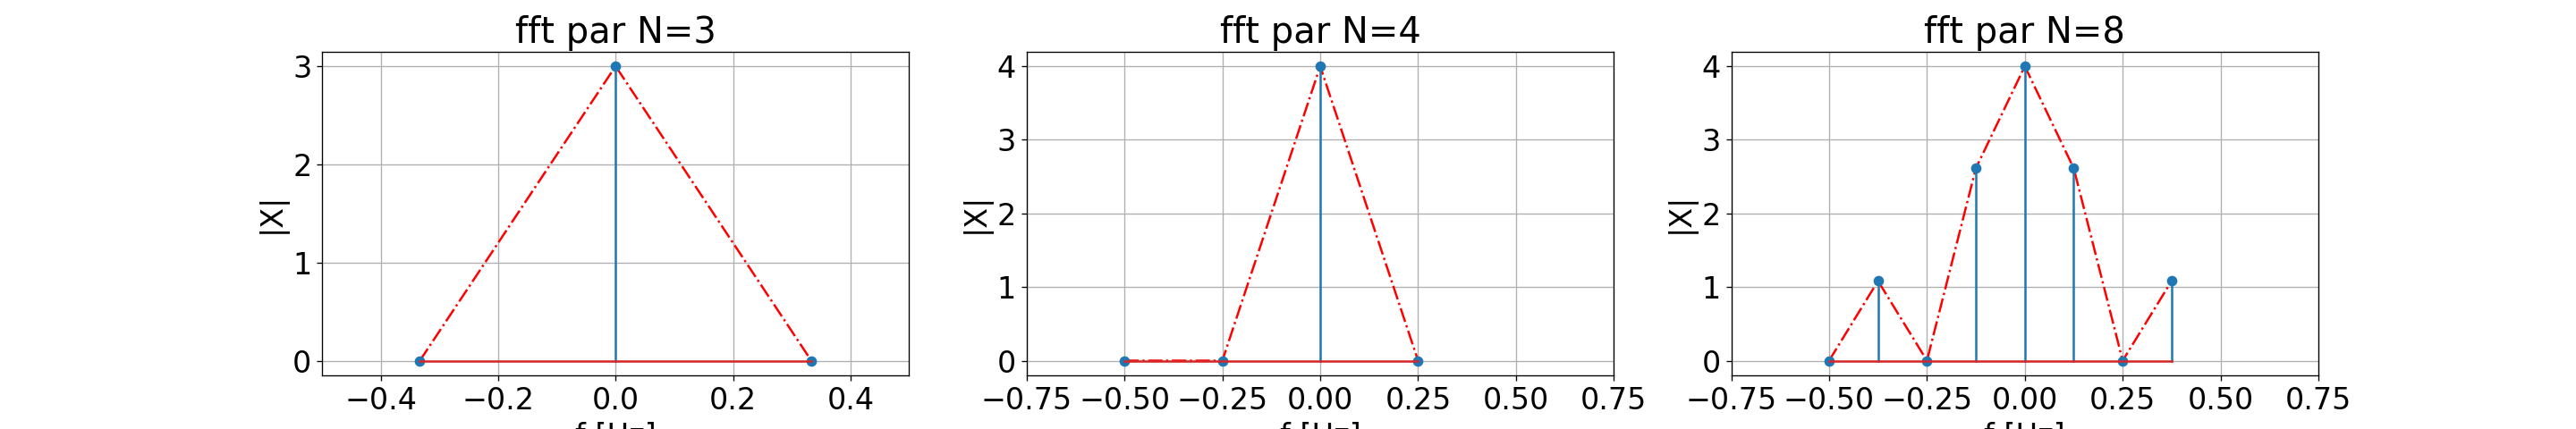
\includegraphics[width=\textwidth]{Img/punto_3_b.png}
\caption{Espectros generados con 3,4 y 8 puntos.}
\label{fig.3b}
\end{figure}

Se añadio en los graficos una señal punteada que corresponde al espectro real de la señal $x[n]$.
Se puede apreciar que los valores que toma la DFT coinciden con el valor de la envolvente en dichos puntos, por lo que seria posible aproximar la DTFT con la DFT.


\end{document}